On completion of the implementation of all the modules presented in the previous sections, we compared the machine's behavior in different applications.\\
There were three test configurations:
\begin{itemize}
	\item Kinematic linearizer + Gazebo Physics
	\item Kinematic linearizer + ODE Physics
	\item Kinematic linearizer + Gazebo Physics + Pacejka friction model 
\end{itemize}
The experimental results obtained were consistent with theoretical expectations. \\
In this chapter, we illustrate two general considerations from the execution of each test case.

\subsection{Original Gazebo model vs. ODE model}
As it turned out, with the same modules applied, these two models gave very similar results.\\
This is due to the fact that the Gazebo simulator uses the ODE (Open Dynamics Engine) library as its physics engine to simulate rigid-body dynamics.\\
Since these two models are based on the same physics engine, there were no differences during the application.

\begin{figure}[H]
	\includegraphics[width=\textwidth]{gazebo_sim.png}
	\caption{The eight trajectory simulated using Gazebo Physics model}
\end{figure}

\begin{figure}[H]
	\includegraphics[width=\textwidth]{ode_sim.png}
	\caption{The eight trajectory simulated using ODE Physics model}
\end{figure}


\subsection{Pacejka friction model}
The testing phase of the Pacejka module provided results consistent with what was expected from the theory. By defining the graphs between force and slip, it can be seen that the data collected takes the form of a sigmoid function.\\
Theoretically, Pacejka's application and the related machine behaviour are consistent. \\
Since no empirical data is available, we cannot ascertain whether our model works optimally. To be able to compare the different models, we would need a basic model to refer to and set as ground truth.\\
The results presented below were collected by applying the eight trajectory.

\begin{figure}[H]
	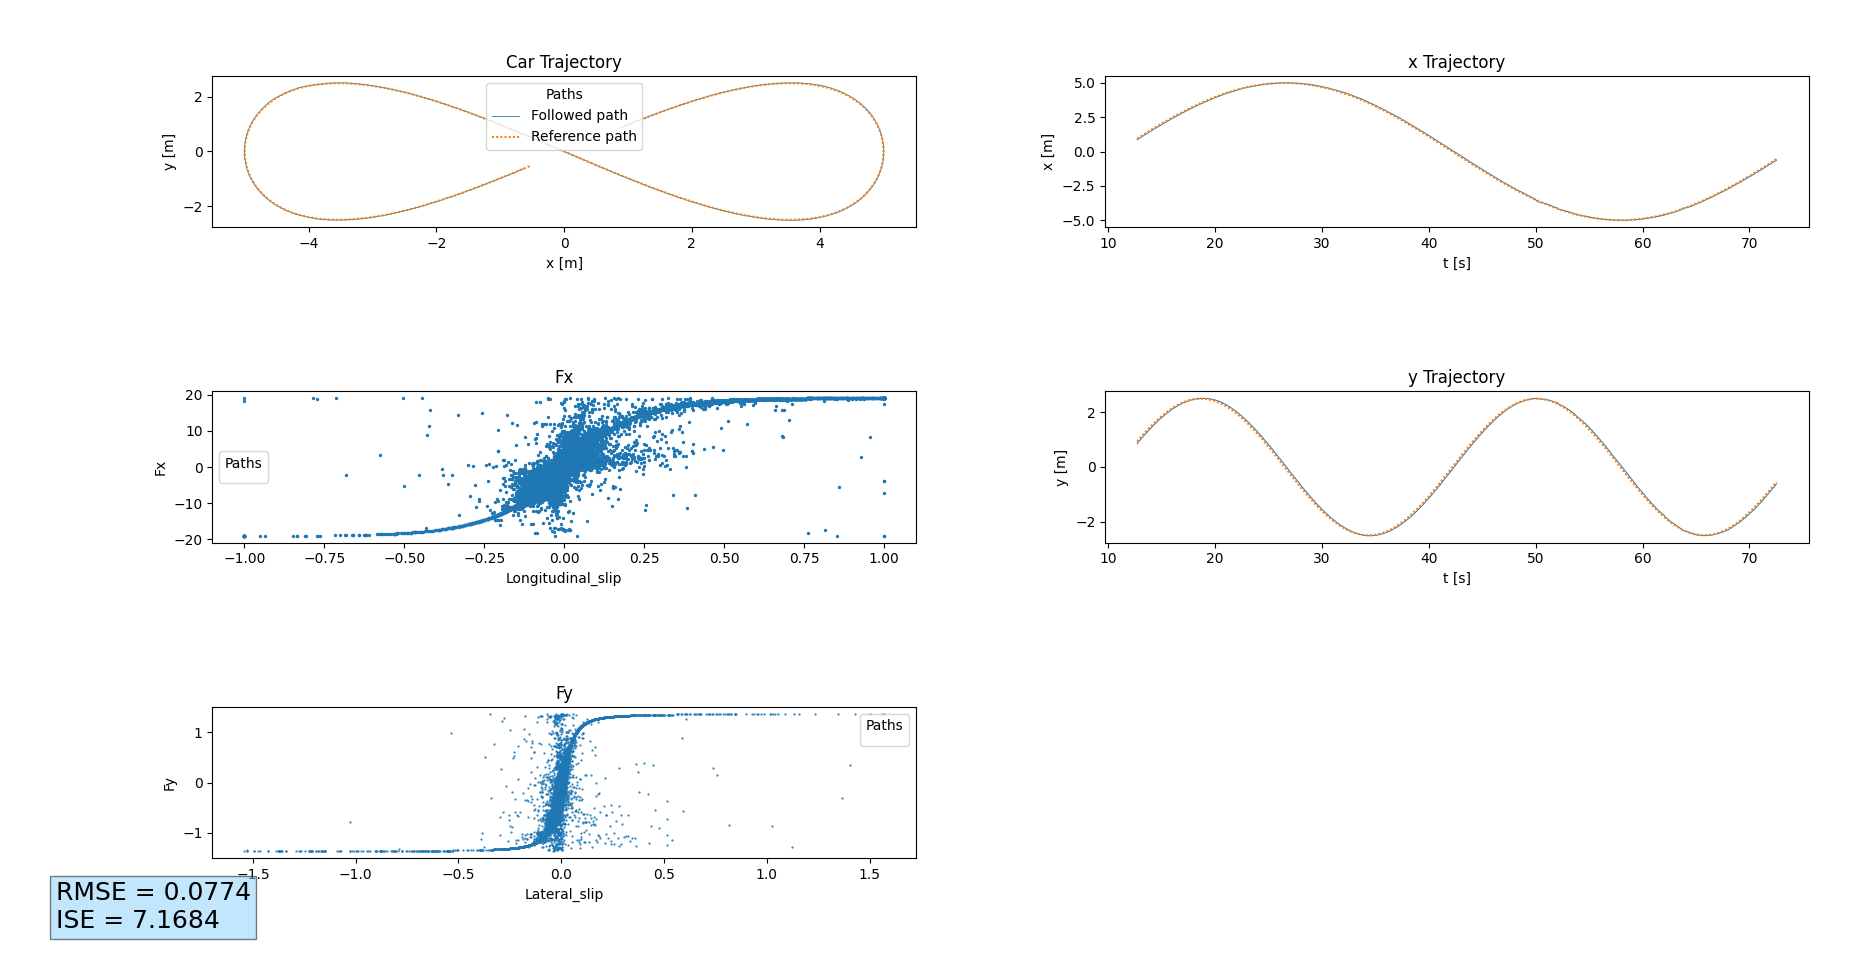
\includegraphics[width=\textwidth]{eight_sim.png}
	\caption{The eight trajectory simulated using Pacejka friction and Gazebo physics models}
\end{figure}

We would also like to present the results obtained by applying the Pacejka modulus correlated with the machine's rectilinear trajectory. \\
As can be seen from the force graph, the values are scattered and not as precise as in the case of the eight trajectory. The reason is related to the parameters used in the calculation of the Pacejka formula. The values chosen were experimentally tested on the eight trajectory, as specified in the section on the plugin.
\begin{figure}[H]
	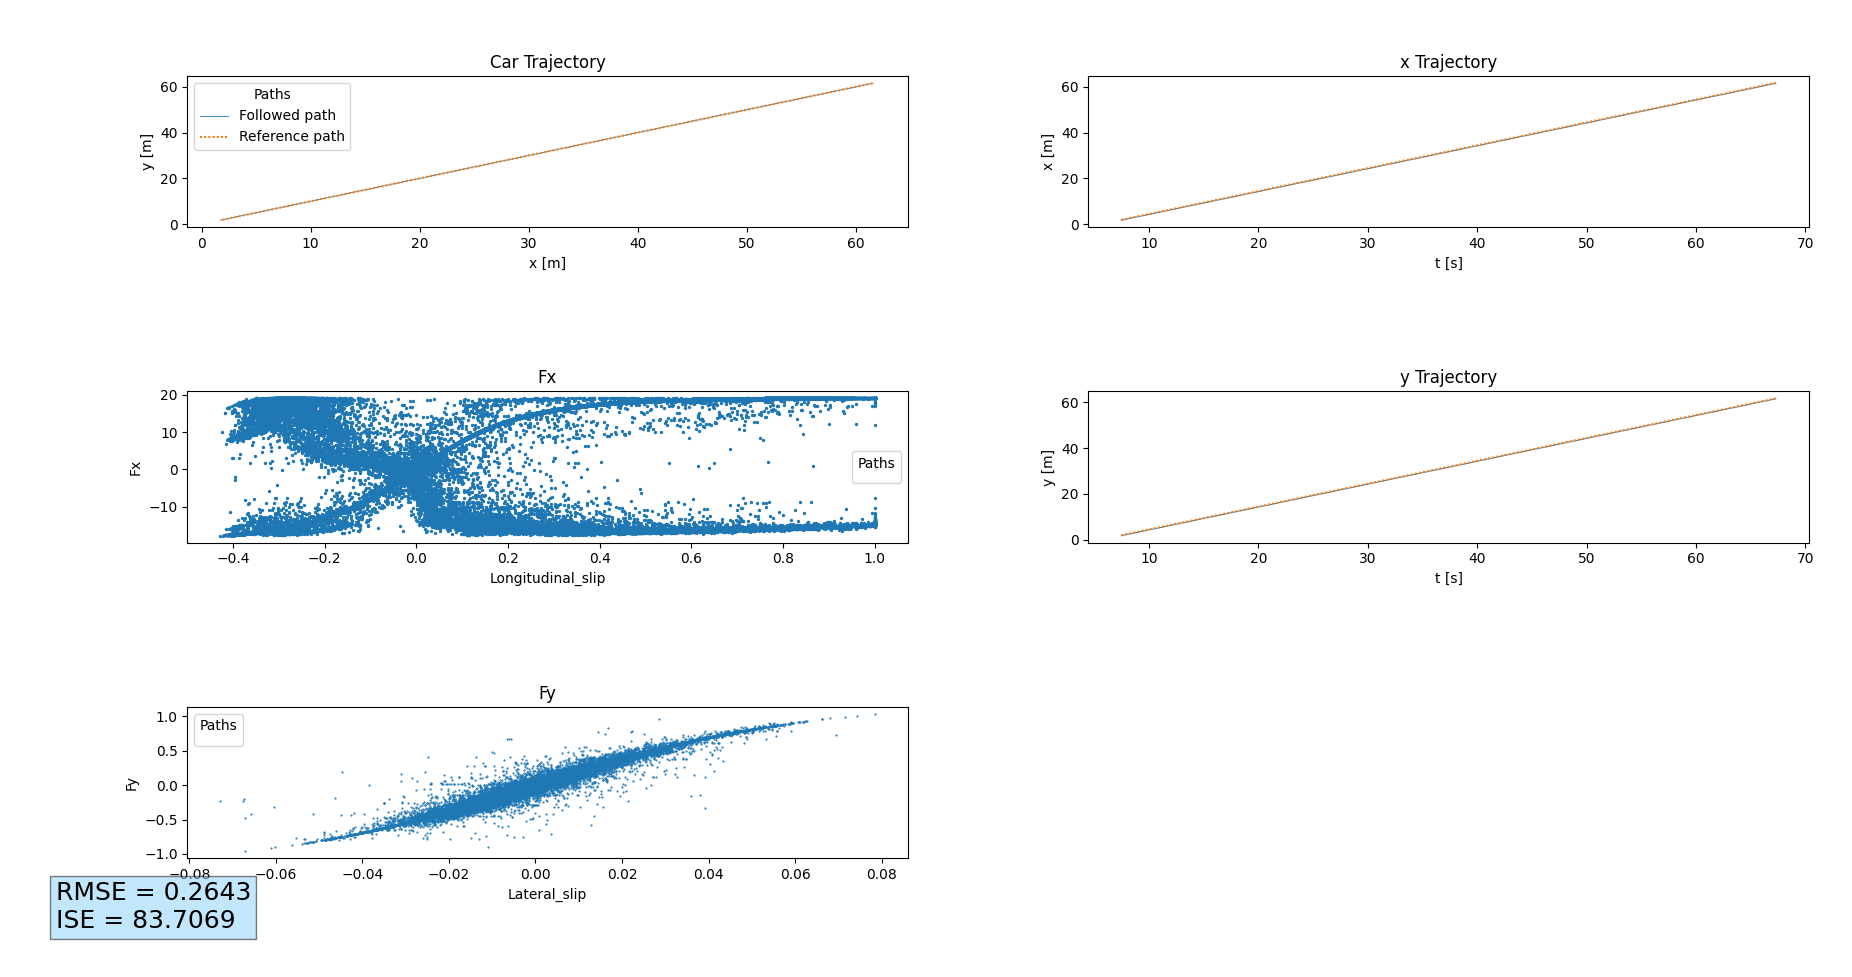
\includegraphics[width=\textwidth]{rect_sim.png}
	\caption{The rectilinear trajectory simulated using Pacejka friction and Gazebo physics models}
\end{figure}